\section{冻结控制器的最终留出测试}
\label{sec:w2-final-test}
\subsection{测试对象与预定比较}

完成模型选择与开发检验后，冻结四类学习控制器及六个简单对照，在未参与开发的1000至1029号环境种子上执行最终测试。十种方法分别覆盖$r=4.4$、4.8以及干净、10\%持续虚假高奖励背叛四个条件，共完成1200次100000步运行。所有方法均从相同种子对应的初始Q表和环境开始，控制器参数不再调整，没有提前停止或按结果删除运行。

主要指标为全程平均合作率，也是本环境的标准化全程真实福利。测试前规定八项主要比较：在四个条件中，完整模型分别减去调好强度的固定合作规则，以及固定合作评分下学习门控。以环境种子为单位进行100000次配对bootstrap，同一个重采样索引同时用于各方法和四个条件。逐比较报告95\%百分位区间，并对八项比较报告Bonferroni校正后的99.375\%百分位区间。后者是近似bootstrap区间，不是任意分布下的精确有限样本保证。

以下标准差描述30次独立环境运行的差异，区间描述冻结控制器之间的平均配对差。它们不包含重新训练的全部不确定性；独立优化重复及未选中的候选已在表\ref{tab:w2-training-repeats}中另行列出。

\subsection{相对固定规则的收益与评分学习的增量}

表\ref{tab:w2-final-whole}汇总各方法的全程合作。在两个受扰条件下，完整模型分别达到0.96774和0.98398，固定合作规则为0.92044和0.94213。干净条件下，完整模型分别为0.97261和0.98298，同样高于该固定规则。这说明在已规定的四个条件中，训练所得的信息控制提供了超出固定合作偏好的收益。

\begin{table}[!htbp]
\centering\small
\caption{最终测试的全程合作均值与运行间标准差}
\label{tab:w2-final-whole}
\begin{tabular}{clrr}
\toprule
$r$ & 方法 & 干净 & 10\%持续失真 \\
\midrule
4.4 & 完整模型 & $0.97261\pm0.00012$ & $0.96774\pm0.00033$ \\
4.4 & 固定评分/学习门控 & $0.96831\pm0.00018$ & $0.96115\pm0.00016$ \\
4.4 & 学习评分/固定门控 & $0.95329\pm0.00019$ & $0.94173\pm0.00138$ \\
4.4 & 最高奖励/学习门控 & $0.96460\pm0.00021$ & $0.46749\pm0.02064$ \\
4.4 & 独立Q-learning & $0.38279\pm0.00034$ & $0.38279\pm0.00034$ \\
4.4 & 全局NI & $0.77478\pm0.30668$ & $0.03470\pm0.04429$ \\
4.4 & 局部NI & $0.37468\pm0.42743$ & $0.00569\pm0.00004$ \\
4.4 & 上尾过滤 & $0.03079\pm0.13745$ & $0.31122\pm0.35595$ \\
4.4 & 固定合作规则 & $0.92006\pm0.00007$ & $0.92044\pm0.00007$ \\
4.4 & 幅度校准固定规则 & $0.79241\pm0.00071$ & $0.69697\pm0.02686$ \\
\midrule
4.8 & 完整模型 & $0.98298\pm0.00003$ & $0.98398\pm0.00010$ \\
4.8 & 固定评分/学习门控 & $0.98515\pm0.00004$ & $0.98398\pm0.00005$ \\
4.8 & 学习评分/固定门控 & $0.97501\pm0.00004$ & $0.97371\pm0.00083$ \\
4.8 & 最高奖励/学习门控 & $0.98253\pm0.00007$ & $0.71314\pm0.01093$ \\
4.8 & 独立Q-learning & $0.45511\pm0.00146$ & $0.45511\pm0.00146$ \\
4.8 & 全局NI & $0.93871\pm0.00193$ & $0.12475\pm0.03694$ \\
4.8 & 局部NI & $0.72089\pm0.36273$ & $0.00578\pm0.00004$ \\
4.8 & 上尾过滤 & $0.87766\pm0.16466$ & $0.80582\pm0.01277$ \\
4.8 & 固定合作规则 & $0.94193\pm0.00004$ & $0.94213\pm0.00005$ \\
4.8 & 幅度校准固定规则 & $0.84175\pm0.00048$ & $0.83337\pm0.00053$ \\
\bottomrule
\end{tabular}
\par\smallskip{\zihao{-5}\rmfamily 来源：作者，本文冻结后的留出测试，每个条件30次独立运行，2026年。\par}
\end{table}


表\ref{tab:w2-final-primary}进一步给出配对差。在四个条件中，完整模型相对固定合作规则的全程优势为4.105至5.255个百分点，八项校正中对应的四个区间均位于零以上。例如，$r=4.4$受扰条件的优势为4.7305个百分点，校正区间为$[4.7144,4.7468]$；$r=4.8$受扰条件的优势为4.1851个百分点，校正区间为$[4.1797,4.1904]$。这些估计对应固定参数在指定环境中的重复表现，不扩展为整个协同因子区间的结论。

\begin{table}[!htbp]
\centering\small
\caption{最终测试的主要全程合作配对差及bootstrap区间，单位为百分点}
\label{tab:w2-final-primary}
\begin{tabular}{cclrrr}
\toprule
$r$ & 异常比例 & 对照 & 均值差 & 95\%区间 & 99.375\%区间 \\
\midrule
4.4 & 0\% & 固定合作规则 & 5.255 & [5.250, 5.260] & [5.248, 5.262] \\
4.4 & 0\% & 固定评分门控 & 0.430 & [0.422, 0.438] & [0.420, 0.441] \\
4.4 & 10\% & 固定合作规则 & 4.730 & [4.719, 4.742] & [4.714, 4.747] \\
4.4 & 10\% & 固定评分门控 & 0.659 & [0.647, 0.672] & [0.642, 0.677] \\
4.8 & 0\% & 固定合作规则 & 4.105 & [4.103, 4.107] & [4.102, 4.107] \\
4.8 & 0\% & 固定评分门控 & -0.217 & [-0.218, -0.216] & [-0.219, -0.216] \\
4.8 & 10\% & 固定合作规则 & 4.185 & [4.181, 4.189] & [4.180, 4.190] \\
4.8 & 10\% & 固定评分门控 & -0.000 & [-0.004, 0.003] & [-0.005, 0.004] \\
\bottomrule
\end{tabular}
\par\smallskip{\zihao{-5}\rmfamily 来源：作者，本文冻结后的留出测试，每个条件30次独立运行，2026年。\par}
\end{table}


学习评分的额外作用则较小，并且随条件改变。$r=4.4$时，完整模型相对固定评分门控的干净、受扰优势分别为0.4302和0.6594个百分点，相应校正区间均为正。$r=4.8$干净条件下，完整模型反而低0.2173个百分点，校正区间为$[-0.2189,-0.2158]$；受扰条件下的差接近零，校正区间为$[-0.0052,0.0045]$。后一结果不足以支持完整模型更高，也不能仅凭区间跨零就证明两种方法等效。

因此，最终测试支持两个不同层次的判断：相对已调好的固定合作规则，学习控制在本次四条件中均有收益；相对固定合作评分加学习门控，进一步学习评分只在部分条件中提供增量。固定评分结构只有七个可训练门控参数，已解释大部分提升。将全部改善都归功于复杂消息评分，会掩盖这个更简单对照的作用。

\subsection{学习轨迹、末段水平与运行分布}

图\ref{fig:w2-final-trajectories}展示六种代表方法的平均轨迹，全部十种方法的数值均保留在表格和逐次结果中。完整模型与固定评分门控在所示条件下较早进入高合作区间；全局NI在干净条件下可出现先下降、后恢复，而受到持续高奖励背叛报告后保持低合作。这里每个点是100步分段均值再对30次运行平均，不能将平滑后的曲线当作某一次运行的轨迹。

\begin{figure}[!htbp]
\centering

\includegraphics[width=\linewidth]{figures/work2-final/trajectories.pdf}
\caption{最终测试的平均合作轨迹。横轴为对数步号，每条曲线平均30次独立运行；固定合作规则取$\kappa=0.2$。其余方法的全程与末段指标在完整表格中报告。}
\label{fig:w2-final-trajectories}
\par\smallskip{\zihao{-5}\rmfamily 来源：作者，本文冻结后的留出测试，每个条件30次独立运行，2026年。\par}
\end{figure}

在$r=4.8$时，全局NI的末段合作均值从干净条件下的0.94500降到受扰条件下的0.12940，完整模型对应为0.98335和0.98443。受扰时，最高奖励选择加学习门控的末段均值为0.71329，仅学习评分而固定门控为0.4时为0.97443。这个结构对照与第四章的方向分析一致：调小既定背叛参考的影响，不能直接把该修正转为合作方向；参考选择与幅度控制的组合仍需共同评价。

均值还必须结合运行分布解释。图\ref{fig:w2-final-tail-distribution}显示，在$r=4.4$的干净条件下，全局NI的末段均值为0.78733，但逐次值分布在约0.006与0.91附近；局部NI的均值为0.37952，也不是大多数运行的典型水平。上尾过滤在$r=4.4$受扰时同样呈现高低合作分离，其末段均值为0.33912、标准差为0.38687。相比之下，完整模型在两个受扰条件的末段标准差分别为0.000415和0.000135，本批30次运行均集中在较高合作区间。

\begin{figure}[!htbp]
\centering
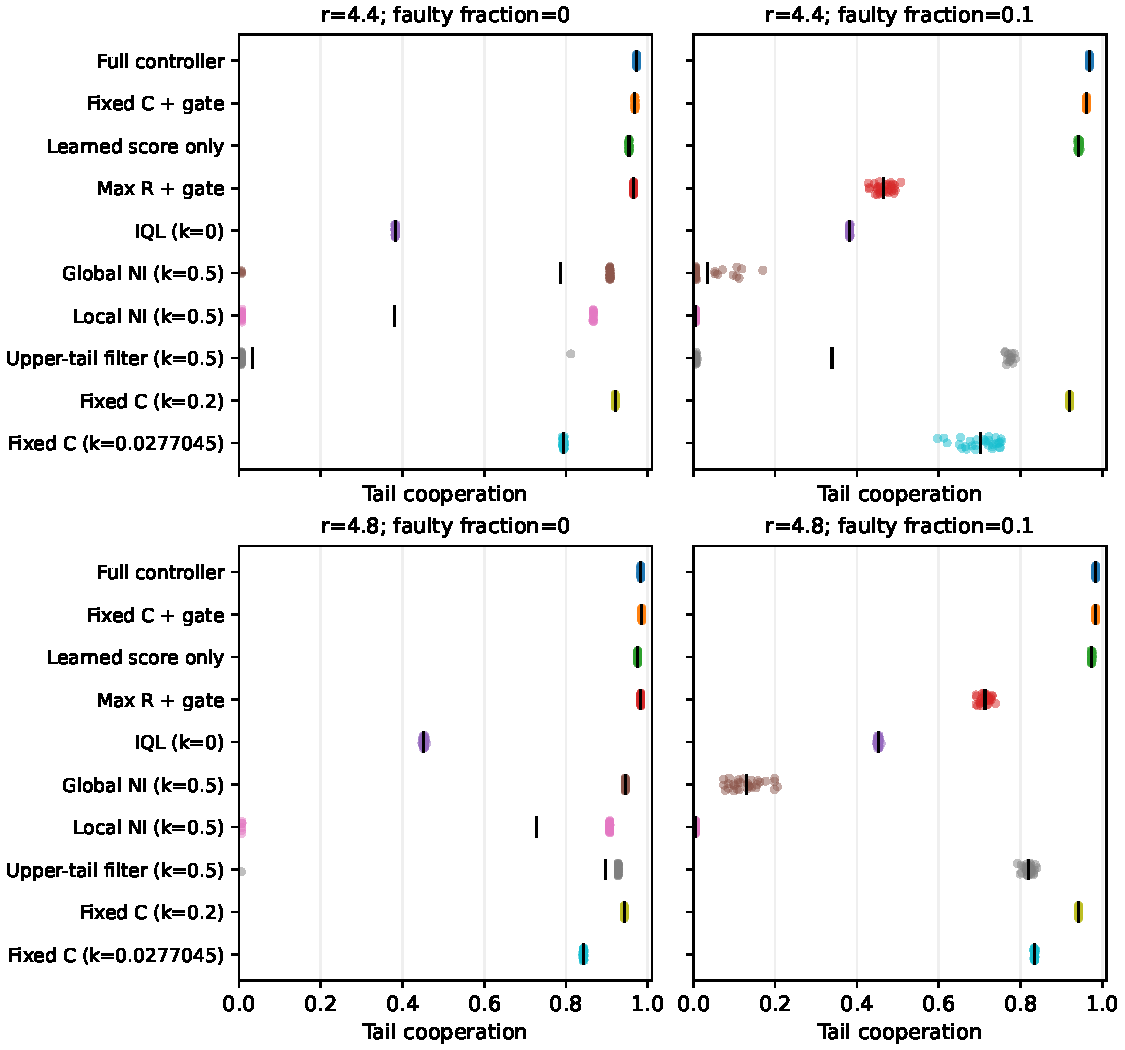
\includegraphics[width=\linewidth]{figures/work2-final/distributions-tail.pdf}
\caption{最终测试的全部末段合作值。每种方法、每个条件有30个点，黑色竖线为均值；纵向轻微偏移仅为区分运行。点的数量以独立运行计，不以节点或时间步计。}
\label{fig:w2-final-tail-distribution}
\par\smallskip{\zihao{-5}\rmfamily 来源：作者，本文冻结后的留出测试，每个条件30次独立运行，2026年。\par}
\end{figure}

完整模型在$r=4.4$和4.8受扰时，末段策略切换率仍分别约为0.02599和0.01841。高合作因而没有消除持续探索和动作变化，固定100000步也不能作为吸收态或理论收敛的证明。完整末段均值表与全程逐次分布见附录\ref{app:final-supplement}。

\subsection{参考来源与实际更新幅度}

表\ref{tab:w2-final-mechanism}按全程口径报告受扰时的信息使用。全局NI约有72.193\%的接收者轮次选中异常发送者，接近其候选集合受到异常来源覆盖的水平。完整模型、固定评分门控和固定合作规则的相应比例均低于0.001\%。这个共同现象很重要：简单合作优先同样会避开持续报告背叛的异常来源，低异常选择比例不能单独证明学习控制器掌握了消息真伪。

\begin{table}[!htbp]
\centering\small
\caption{最终测试受扰条件下的信息使用；各项为30次全程指标的均值}
\label{tab:w2-final-mechanism}
\begin{tabular}{clrrrr}
\toprule
$r$ & 方法 & 异常来源/\% & 门控均值 & NI触发/\% & 绝对NI \\
\midrule
4.4 & 完整模型 & $<0.001$ & 0.179 & 20.779 & 0.01316 \\
4.4 & 固定评分门控 & $<0.001$ & 0.176 & 36.891 & 0.02137 \\
4.4 & 全局NI & 72.193 & 1.000 & 79.833 & 0.34732 \\
4.4 & 固定合作规则 & $<0.001$ & 1.000 & 65.779 & 0.08118 \\
4.4 & 幅度校准固定规则 & 0.035 & 1.000 & 83.186 & 0.01075 \\
\midrule
4.8 & 完整模型 & $<0.001$ & 0.172 & 13.948 & 0.01019 \\
4.8 & 固定评分门控 & $<0.001$ & 0.142 & 16.296 & 0.01065 \\
4.8 & 全局NI & 72.193 & 1.000 & 91.976 & 0.35649 \\
4.8 & 固定合作规则 & $<0.001$ & 1.000 & 52.221 & 0.07659 \\
4.8 & 幅度校准固定规则 & $<0.001$ & 1.000 & 79.558 & 0.01304 \\
\bottomrule
\end{tabular}
\par\smallskip{\zihao{-5}\rmfamily 来源：作者，本文冻结后的留出测试，每个条件30次独立运行，2026年。\par}
\end{table}


完整模型在$r=4.4$、4.8受扰时的门控均值分别约为0.179和0.172，实际NI触发比例分别为20.779\%和13.948\%。两类数值含义不同：门控是连续系数，触发还要求选中报告具有正奖励优势。完整模型的平均绝对NI约为0.01316和0.01019，低于固定合作规则的0.08118和0.07659；但不能只由这个差异断言较弱更新就是高合作的唯一原因。

幅度校准固定规则在最终四条件中的汇总绝对NI为0.01295，完整模型为0.01248，相对差约3.79\%，而其两个受扰条件的全程合作仅为0.69697和0.83337。开发阶段选定的固定强度在这里保持不变。这个补充说明，较接近的汇总更新量仍不足以获得相同合作过程；同时它仍未控制逐条件幅度、触发时机、空间位置和策略轨迹，因此不构成某一个特征的独立因果贡献估计。

图\ref{fig:w2-final-snapshot}给出预先指定的1000号种子在$r=4.8$受扰条件下的末轮动作。两类学习控制器与固定合作规则均保留较多合作，最高奖励全局NI则以背叛为主。这一示例与总体统计相符，但图中的900个节点不是900次独立验证。$r=4.4$下同一种子的对应快照也在附录中保留，未按视觉效果更换种子。

\begin{figure}[!htbp]
\centering
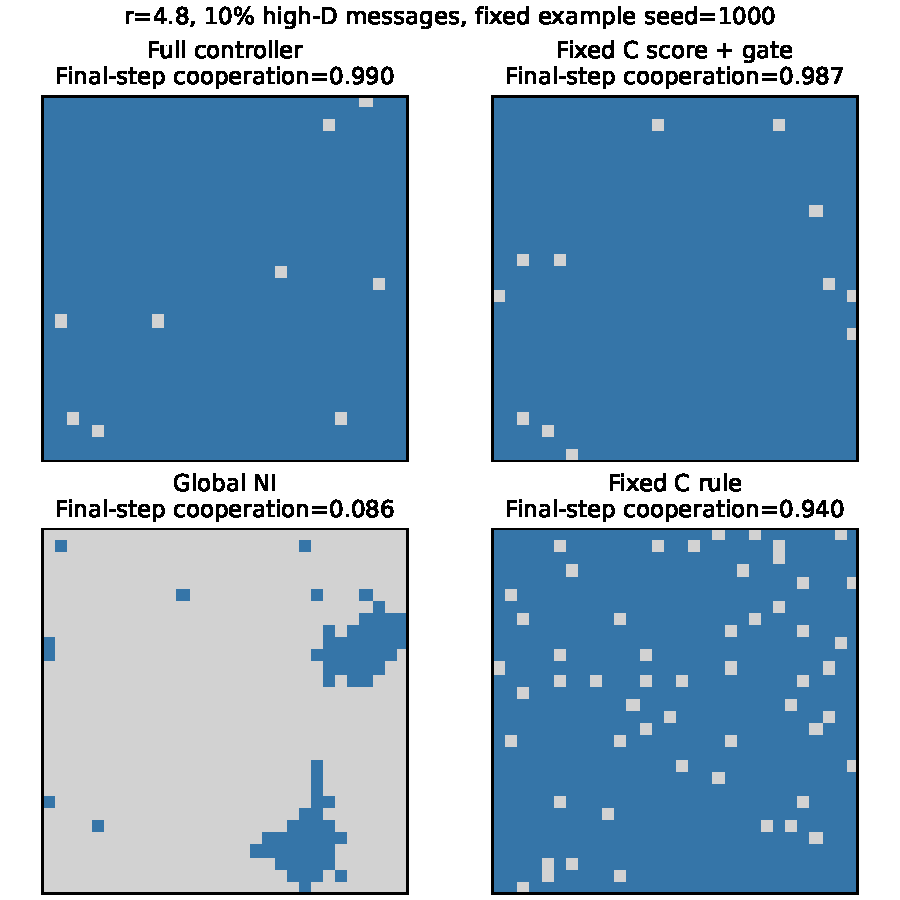
\includegraphics[width=.88\linewidth]{figures/work2-final/snapshots-r4.8.pdf}
\caption{最终测试中预定种子1000的末轮真实动作，$r=4.8$、10\%持续失真。蓝色表示合作，灰色表示背叛；图中比例为该末轮快照值，不是末段平均。}
\label{fig:w2-final-snapshot}
\par\smallskip{\zihao{-5}\rmfamily 来源：作者，本文冻结后的留出测试，每个条件30次独立运行，2026年。\par}
\end{figure}

所有1200条配置与输出均通过核验，包括Q表和异常掩码散列、分段轨迹与全程及末段汇总的对应，以及真实福利恒等式。以上结论首先属于该冻结版本、两种协同因子和指定消息通道；下文的开发机制检验与泛化结果用于解释这些表现及其适用边界。
